% !Mode\dots ``TeX:UTF-8''
% !TEX root = ../bare_jrnl.tex


\section{The online observability of \BCNs}
\label{sec:online}

%In this section we propose the online observability to solve the problem mentioned in {\em Section \ref{sec:pre}}, and we will introduce its related information in detail. 
%
%In the rest of this section, firstly we introduce the inspiration for the online observability. Secondly we define derivation function. Thirdly we present the definition of $k$-step determinability. Finally, we give the formal definition of the online observability of \BCNs\ by derivation function and $k$-step determinability, and compare it with four existing observability.

%\subsection{Inspiration}


As we mentioned in {\em Section \ref{sec:pre}}, we can determine the initial states of \BCNs\ by the third existing observability. But in the third observability, a \BCN\ is observable iff \tl{unless?} there exists an finite input sequence $\mathsf{I}\in(\Delta_M)^k$ that determine its initial state $\mathsf{s}(0)$. 

However, as we can derive the set of possible initial states $\mathsf{S}(0)$ by initial output $\mathsf{o}(0)$ we observe
\[\mathsf{S}(0)=\{\mathsf{s}(0)|\mathsf{s}(0)\in \Delta_N\ ,\ h( \mathsf{s}(0))=\mathsf{o}(0)\}.\]
And if for every $\mathsf{S}^{i}(0)$ (corresponding to the $\mathsf{o}^{i}(0)$) we derived, there is an input sequence $\mathsf{I}^{i}\in(\Delta_M)^k$ for some $k>0$, such that for any distinct states $\mathsf{s}^{x}(0)$, $\mathsf{s}^{y}(0) \in \mathsf{S}^{i}(0)$ implies $(HF)^k_{\mathsf{s}^{x}(0)}(\mathsf{I^i})\neq (HF)^k_{\mathsf{s}^{y}(0)}(\mathsf{I^i})$,
then we can determine the initial state too. 
What is more, in this case, the requirements for a \BCN\ to determine its initial state would be easier to meet. Because the corresponding input sequences $\mathsf{I}^{i}$ of different sets of possible initial states $\mathsf{S}^{i}(0)$ can be different. While in the third existing observability the $\mathsf{I}^{i}$ has to be identical.

Furthermore, we can derive the set of possible states $\mathsf{S}(1)$ by the outputs $\mathsf{o}(0)$ and $\mathsf{o}(1)$ we observe and the input $\mathsf{i}(0)$ 
\[\mathsf{S}(1)=\{\mathsf{s}(1)|\mathsf{s}(0)\in \mathsf{S}(0),\ \mathsf{s}(1)=f({\mathsf{i}(0)},{\mathsf{s}(0)}),\ h(\mathsf{s}(1))=\mathsf{o}(1)\}.\]

And if for every $\mathsf{S}^{i}(1)$ we derived, 
\begin{itemize}
  \item  there is an input sequence $\mathsf{I}^{i}\in(\Delta_M)^k$ for some $k>0$, such that for any distinct states $\mathsf{s}^{x}(1)$, $\mathsf{s}^{y}(1) \in \mathsf{S}^{i}(1)$ implies $(HF)^k_{\mathsf{s}^{x}(1)}(\mathsf{I^i})\neq (HF)^k_{\mathsf{s}^{y}(1)}(\mathsf{I^i})$;
  \item  and for every $\mathsf{s}^{x}(1)$ $\in \mathsf{S}^{i}(1)$ there exists only one corresponding $\mathsf{s}^{x}(0)$ $\in \mathsf{S}^{i}(0)$ such that $\mathsf{s}^{x}(1)=f({\mathsf{i}(0)},{\mathsf{s}^{x}(0)})$,
\end{itemize} 
then we can determine the initial state too. And in this case, the requirements for the \BCN\ to determine the initial state would be further easier to meet. Because the corresponding input sequences $\mathsf{I}^{i}$ of different sets of possible states $\mathsf{S}^{i}(1)$ can be different. 

Therefore, we have that if we utilize sets of possible states we derived more, it would be easier for a \BCN\ to meet the requirements to determine its initial state. According to this rule, we propose the online observability. Instead of finding the input sequence $\mathsf{I}$ before we take the procedure of determining the initial state. In the online observability we use the $\mathsf{S}(t)$ (which will be formally defined in the next subsection) we derive at every time step to adaptively contruct the input sequence to determine the initial state of \BCNs. Such that the requirements to determine the \BCNs' initial state would be easiest to meet. Thus, a \BCN\ satisfies the online observability iff its initial state $\mathsf{s}(0)$ can be determined for every $\mathsf{s}(0) \in \Delta_N$.

After introducing the idea of the online observability, we briefly present how to determine the initial state of a \BCN. At every time setp $t$, 
\begin{itemize}
\item firstly, we observe the output $\mathsf{o}(t)$ of \BCN, then based on the relation $\mathsf{o}(t)=h(\mathsf{s}(t))$ we can infer the set of possible states $\mathsf{S}(t)$ by the $\mathsf{o}(t)$.
\item Secondly, with the set of possible states $\mathsf{S}(t)$ we can derive the set of possible inputs $\{\mathsf{i}_z(t),\ldots,\mathsf{i}_w(t)\}$, such that for every $\mathsf{i}^{i}(t)\in \{\mathsf{i}_z(t),\ldots,\mathsf{i}_w(t)\}$ we have  for any distinct $\mathsf{s}^{x}(t)$, $\mathsf{s}^{y}(t) \in \mathsf{S}(t)$, they will not become the same state after being affected by this input $\mathsf{i}^{i}(t)$ i.e., $f(\mathsf{s}^{x}(t), \mathsf{i}^{i}(t))\neq f(\mathsf{s}^{y}(t),\mathsf{i}^{i}(t))$.  And then, we choose an input $\mathsf{i}(t)$ from $\{\mathsf{i}_z(t),\ldots,\mathsf{i}_w(t)\}$.
\item Thirdly, based on the relation $\mathsf{s}(t+1)= f({\mathsf{i}(t)},{\mathsf{s}(t)})$, the set of possible states $\mathsf{S}(t+1)$ of next time step ($t+1$) is preliminarily derived. 
\end{itemize} 

 The cardinal number of possible states set does not change or decrease in the determining process i.e. $|\mathsf{S}(t+1)|\le|\mathsf{S}(t)|$. % (will be shown in {\em Example \ref{exa:8}}). 
 If the cardinal number of possible states set $|\mathsf{S}(t)|=1$, then we can determine the $\mathsf{s}(t)$. And then because for every $\mathsf{s}^{i}(t)\in $ $\mathsf{S}(t)$ there is exact one corresponding $\mathsf{s}^{i}(t-1)\in $ $\mathsf{S}(t-1)$, we can determine $\mathsf{s}(t-1)$, $\mathsf{s}(t-2)$, \ldots, and $\mathsf{s}(0)$.

Therefore, in the definition of online observability, 
\begin{itemize}
\item firstly we need to describe how to derive the set $\mathsf{S}(t)$ of possible states of the \BCN\ by the output $\mathsf{o}(t)$, input $\mathsf{i}(t-1)$ and $\mathsf{S}(t-1)$. So we define the derivation function to solve this problem.
\item  Secondly, we need to describe how to derive the $\mathsf{i}(t)$ to determine $\mathsf{s}(0)$ by the $\mathsf{S}(t)$. Thus we define the $k$-step determinability for $\mathsf{S}(t)$ which means that we can determine $\mathsf{s}(t)$ by $\mathsf{S}(t)$ in $k$ time steps.
\end{itemize} 

Therefore, we have the definition of the online observability that a \BCN\ is online observable if for every $\mathsf{S}^{i}(0)$ we derived, there exists a $k^i\ge 0$ such that the $\mathsf{S}^{i}(0)$ is $k^i$-step determinable.


\subsection{Derivation function}

In order to better describe how to derive the set of possible states $\mathsf{S}(t)$ at every time step $t$, we propose the derivation function. The definition of it is as follows.

\begin{definition}[Derivation Function] 
In a Boolean control network, let
\begin{itemize}
\item $2^{\Delta_N}$ be the power set of states; 
\item $(\Delta_M\cup\varepsilon)$ be the set of inputs and $\varepsilon$ means empty input; 
\item $(\Delta_Q\cup\varepsilon)$ be the set outputs and $\varepsilon$ means empty output.
\end{itemize} 

\[\Ded:2^{\Delta_N}\times (\Delta_M\cup\varepsilon) \times (\Delta_Q\cup\varepsilon) \mapsto 2^{\Delta_N}\] 
is the derivation function that
\begin{equation*}
\begin{split}
&\Ded\left( \mathsf{S},  \mathsf{i},  \mathsf{o}\right)\\
&=\{ \mathsf{s}'| \mathsf{s}'=\left\{
\begin{array}{rcl}
f( \mathsf{i}, \mathsf{s})      &      & {\mathsf{i}\neq \varepsilon}\\
\mathsf{s}       &      & {\mathsf{i}= \varepsilon}
\end{array} \right. ,\ h(\mathsf{s}')=\mathsf{o}\ if\ \mathsf{o}\neq \varepsilon\}.
\end{split}
\end{equation*}

\end{definition}

\begin{example}
 In order to better illustrate the derivation functon $\Ded\left( \mathsf{S},  \mathsf{i},  \mathsf{o}\right)$, we use the \BCN\ mentioned in {\em Example \ref{exa:2}} as an example to apply this function. 
 
 \begin{equation*}
\begin{split}
\Ded\left(\{\delta_{16}^0,\delta_{16}^1,\delta_{16}^2\},\delta_4^0,\delta_4^2\right)=&\{\delta_{16}^{9},\delta_{16}^{10}\}\\
\end{split}
\label{equ:11}
\end{equation*}

If the possible states set $\mathsf{S}=\{\delta_{16}^0$, $\delta_{16}^1$, $\delta_{16}^2\}$ and we input $\delta_4^0$ observe $\delta_4^2$, then we can derive that the set of possible new states can be $\delta_{16}^{9}$ or  $\delta_{16}^{10}$.
 \label{exa:8}
 \end{example}   
 
 Then for a \BCN, we have the set of possible states $\mathsf{S}(t)$ is defined as follows.
 \begin{definition}[$\mathsf{S}(t)$] In a \BCN, with the input sequence $\mathsf{i}(0)\mathsf{i}(1)\ldots\mathsf{i}(k-1)$ and output sequence $\mathsf{o}(0)\mathsf{o}(1)\ldots\mathsf{o}(k)$, for every $0\le t\le k$, we have
	\[\mathsf{S}(t)=\left\{
\begin{array}{rcl}
\Ded\left(\Delta_N,\varepsilon,\mathsf{o}(0)\right)      &      & {t=0}\\
\Ded\left(\mathsf{S}(t-1),\mathsf{i}(t-1),\mathsf{o}(t)\right)       &      & {t>0}
\end{array} \right. \]

\end{definition}
 
 
\subsection{$K$-step determinability}
As the derivation function can only describe the process of deriving the set possible states $\mathsf{S}(t)$ of \BCNs\ at every time step.  We propose the $k$-step determinability for $\mathsf{S}(t)$ to depict whether we can determine the $\mathsf{s}(t)$ in $k$ time steps for every $\mathsf{s}(t)\in \mathsf{S}(t)$. With this notion, we can know how to derive the $\mathsf{i}(t)$ by $\mathsf{S}(t)$ in the process of determining $\mathsf{s}(0)$. 
\begin{definition}[$k$-Step Determinability] 
For a non-empty  set of states $\mathsf{S}$, the $k$-step determinability of it is recursively defined as follows:
 \begin{itemize}
 \item When $k=0$, $\mathsf{S}$ is $0$-step determinable if $|\mathsf{S}|=1$. 
 \item When $k>0$, $\mathsf{S}$ is $k$-step determinable
 if there is an input $\mathsf{i}^{i} \in \Delta_M$ such that
 \begin{itemize}
 \item  $|\Ded\left(\mathsf{S},\mathsf{i}^{i},\varepsilon\right)|=|\mathsf{S}|$, and 
 \item  for each \[\mathsf{o}^{j}\in \Delta_Q\] such that \[\Ded\left(\mathsf{S},\mathsf{i}^{i},\mathsf{o}^{j}\right)\neq \emptyset,\] there exists a ${k'}\le 
(k-1)$ such that $\Ded\left(\mathsf{S},\mathsf{i}^{i},\mathsf{o}^{j}\right)$ is $k'$-step determinable.
 \end{itemize}
 And the $\mathsf{i}^{i}$ is an input which makes $\mathsf{S}$ $k$-step determinable.
 \end{itemize}
\end{definition}

 Then, in order to better illustrate this definition, we give the following example.
\begin{example}
In the \BCN\ mentioned in {\em Example \ref{exa:2}}. If \[\mathsf{o}(0)=\delta_4^0\] then we have \[\mathsf{S}(0)=\Ded\left(\Delta_N,\varepsilon,\delta_4^0\right)=\{\delta_{16}^0,\delta_{16}^1,\delta_{16}^2\},\] the cardinality number of \[\mathsf{S}(0)=|\{\delta_{16}^0,\delta_{16}^1,\delta_{16}^2\}|=3,\] and for this set there exists $\delta_{4}^3$ such that 
 \begin{itemize}
 \item  $|\Ded\left(\{\delta_{16}^0,\delta_{16}^1,\delta_{16}^2\},\delta_{4}^3,\varepsilon\right)|=|\{\delta_{16}^0,\delta_{16}^{13},\delta_{16}^6\}|$,
 \item   and for each $\mathsf{o}^{j}\in \Delta_Q$
  \begin{itemize}
  \item   $\Ded\left(\{\delta_{16}^0,\delta_{16}^1,\delta_{16}^2\},\delta_{4}^3,\delta_{4}^0\right)=\{\delta_{16}^0\}$, that the $\{\delta_{16}^0\}$ is $0$-step determinable;
 \item  $\Ded\left(\{\delta_{16}^0,\delta_{16}^1,\delta_{16}^2\},\delta_{4}^3,\delta_{4}^3\right)=\{\delta_{16}^{13}\}$, that the $\{\delta_{16}^{13}\}$ is $0$-step determable;
  \item  $\Ded\left(\{\delta_{16}^0,\delta_{16}^1,\delta_{16}^2\},\delta_{4}^3,\delta_{4}^1\right)=\{\delta_{16}^{6}\}$, that the $\{\delta_{16}^{6}\}$ is $0$-step determinable.
 \end{itemize}
 \end{itemize}
 Therefore $\mathsf{S}(0)$ is $1$-step determinable, thus we can  input $\delta_{4}^3$ to determine $\mathsf{s}(0)$ at time step $1$.
\label{exa:9}
\end{example}  

In addition, we propose some lemmas for the $k$-step determinability.

\begin{lemma}
For the sets of states $\mathsf{S}^{1}$ and $\mathsf{S}^{2}$, if $\mathsf{S}^{2}$ is $k$-step determinable and $\mathsf{S}^{1}\subseteq \mathsf{S}^{2}$, then $\mathsf{S}^{1}$ is $k$-step determinable.
  \label{lemm:1}
\end{lemma}

Because of the length of the article, we put all the proofs in the {\bf Appendix}. With the {\em Lemma \ref{lemm:1}}, it is easy to propose the {\em Lemma \ref{lemm:2}}
\begin{lemma}
For the sets of possible states $\mathsf{S}^{1}$ and $\mathsf{S}^{2}$, if there exists a $k^{i}\ge 0$ such that $\mathsf{S}^{2}$ is $k^{i}$-step determinable, and $\mathsf{S}^{1}\subseteq \mathsf{S}^{2}$, then there exists a $k^{j}\ge 0$ that $\mathsf{S}^{1}$ is $k^{j}$-step determinable.
\label{lemm:2}
\end{lemma}

The {\em Lemma \ref{lemm:2}} would help us design the algorithm to determine the online observability of a \BCN, and we will represent the details in the {\em Section \ref{sec:deter}}.
%==========================================================================================

\subsection{Online observability}
After the previous preparation, we present the formal definition of the online observability of {\em BCNs} is as follows.

\begin{definition}[Online Observability of  BCNs]
 A \BCN\ is online observable,
if for every \[\mathsf{o}^{j}(0)\in \Delta_Q\] such that \[\Ded(\Delta_N,\varepsilon, \mathsf{o}^{j}(0))\ne \emptyset,\] there exists a $k^{j}\ge0$ such that $\Ded\left(\Delta_N,\varepsilon,\mathsf{o}^{j}(0)\right)$ is $k^{j}$-step determinable.
\end{definition}

 In order to better illustrate the definition of online observability, we give the following example.

\begin{example}
In the \BCN\ mentioned in {\em Example \ref{exa:2}}.  We have that:
 \begin{itemize}
 \item $\Ded\left(\Delta_N,\varepsilon, \delta_{4}^0\right)=\{\delta_{16}^0,\delta_{16}^1,\delta_{16}^2\}$, and it is $1$-step determinable;
 \item $\Ded\left(\Delta_N,\varepsilon, \delta_{4}^1\right)=\{\delta_{16}^3,\delta_{16}^4,\delta_{16}^5,\delta_{16}^6\}$, and it is $1$-step determinable;
 \item $\Ded\left(\Delta_N,\varepsilon, \delta_{4}^2\right)=\{\delta_{16}^7,\delta_{16}^8,\delta_{16}^{9},\delta_{16}^{10}\}$, and it is $2$-step determinable;
 \item $\Ded\left(\Delta_N,\varepsilon, \delta_{4}^3\right)=\{\delta_{16}^{11},\delta_{16}^{12},\delta_{16}^{13},\delta_{16}^{14},\delta_{16}^{15}\}$, and it is $2$-step determinable.
 \end{itemize}
 
Therefore we have this \BCN\ is the online observable, and then we can determine the initial state of this \BCN\ by online observability. Comparing with {\em Example \ref{exa:6}} and {\em Example \ref{exa:7}}, we can use online observability to determine the initial states of some \BCNs\ which can not be determined by existing observability. Thus with the online observability we can research the \BCNs\ better.
\label{exa:10}
\end{example}  

With the defininition of online observability of \BCNs, we have the implication relationships between four existing observability and online observability.

\begin{lemma}
The online obervability implies the existing first observability.
\label{lemm:3}
\end{lemma}

With the existing first observability, we can distinguish every $\mathsf{s}^{i}(0)$ from other types of initial state, and we can also do this by the online obervability. Thus the online obervability implies the existing first observability. 

\begin{lemma}
The existing third observability implies the online obervability.
\label{lemm:4}
\end{lemma}

In the existing third observability, we can determine the initial state $\mathsf{s}^{i}(0)$ of \BCN\ too. Thus the existing third observability implies the online obervability.

Moreover, from the implication relationships between the existing four observability which mentioned in the {\em Section \ref{sec:pre}}, we have the implication relationships between four existing observability and online observability is shown in Fig.~\ref{fig:7}.

\begin{figure}[thpb]
      \centering
      \framebox{\parbox{3in}{
		\centerline{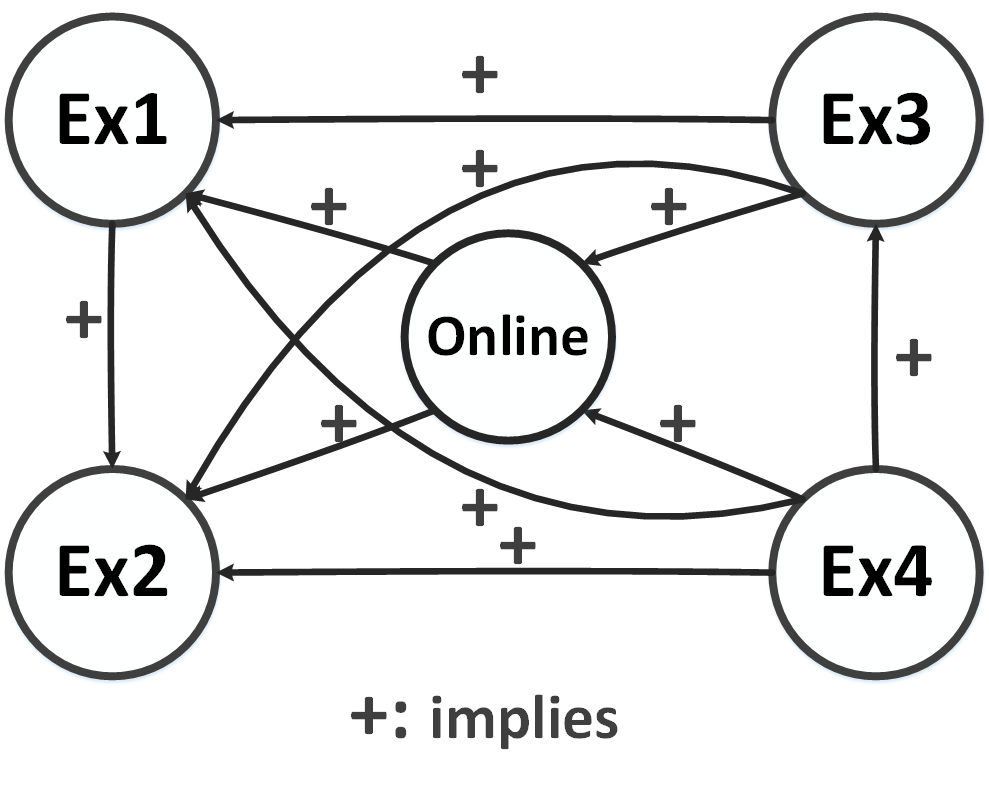
\includegraphics[scale=0.28]{figures/Fig8.png}}
	}}
      
      \caption{The implication relationships graph between existing observability 1, 2, 3, 4, and online observability where ``$\rightarrow$" means ``implies".}
      \label{fig:7}
   \end{figure}


   